\documentclass[10pt, multicolumn, a4paper]{article}

\usepackage{amsmath} % just math
\usepackage{amssymb} % allow blackboard bold (aka N,R,Q sets)
\usepackage{ulem}
\usepackage{enumitem}
\usepackage{tikz}
\setlist{nolistsep}
\usepackage{multicol}
\linespread{1.6}  % double spaces lines
\usepackage[left=1in,top=1in,right=1in,bottom=1in,nohead]{geometry}

\begin{document}

\linespread{1} % single spaces lines
\small \normalsize %% dumb, but have to do this for the prev to work
%\begin{flushright}
%Comp2129
%\end{flushright}

%========================================
% Lecture 2
%========================================

\setcounter{section}{1} % first section is now 2
\hrule
\section{Introduction to C} 
\hrule

\begin{multicols}{2}
	\subsection*{C Modules}
	\begin{itemize}
	\item file translated into obj. file, which gets linked by linker to other object files and std libraries
	\item can refer to global variables/functions of other modules via. externs
	\end{itemize}
	\subsection*{Char input/output}
	\begin{itemize}
	\item \verb|getchar(void)|
	\item \verb|putchar(c)|
	\end{itemize}
	\subsection*{\texttt{printf()} string formats}
	\begin{itemize}
	\item \verb|%.2f| floating pt to 2dp
	\item \verb|%p| pointer
	\end{itemize}
	\subsection*{\texttt{scanf()}}
	\begin{itemize}
	\item reads from std input
	\item returns number of read items
	\item parameters must be pointers
	\end{itemize} 
\end{multicols}

\setcounter{section}{1} % first section is now 2
\hrule
\section{Introduction to Unix}
\hrule 

\begin{multicols}{2}
	\subsection*{\texttt{file}}
	\begin{itemize}
	\item determines type of file
	\item e.g. ordinary, directory, device, 'special'
	\end{itemize}
	\subsection*{Shell environment}
	\begin{itemize}
	\item at login, reads from \verb|/etc/profile|
	\item gets \verb|.bash_profile|, \verb|.profile|
	\end{itemize}
	\subsection*{Permissions}
	\begin{itemize}
	\item user, group, other
	\item read, write, execute
	\item use magical numbers (r: 4, w: 2, x: 1)
	\end{itemize}
	\subsection*{Redirections}
	\begin{itemize}
	\item \verb|a.out < data >res 2>errors|
	\item appending: \verb|>>|
	\end{itemize}
	%\subsection*{Pipes}
	%\begin{itemize}
	%\item takes output from last cmd and uses it as input for the next
	%\end{itemize}
	\subsection*{Shell scripts}
	\begin{itemize}
	\item \verb|#!/bin/bash|
	\item default search path \verb|$PATH|
	\item to execute a script, \verb|./scriptname|, otherwise if the current dir is in \verb|$PATH| it can be executed using \verb|scriptname|
	\end{itemize}
	\subsection*{Shell}
	\begin{itemize}
	\item UNIX cmd interpreter
	\item reads in cmds, runs appropriate programs
	\end{itemize}
	\subsection*{I/O redirection}
	\begin{itemize}
	\item when prog runs, 3 std files opened 
		\\ \verb|0| std input \\ \verb|1| std output \\ \verb|2| std error
	\end{itemize}
	\subsection*{Shell variables}
	\begin{itemize}
	\item stored in environment of the program
	\item setting: \verb|VARNAME = value|
	\item using: \verb|$VARNAME|
	\item script arguments: \verb|$1, $2| etc.
	\end{itemize}
	\subsection*{\texttt{if} statement}
	\begin{itemize}
	\item \texttt{if <cmd> \\ then \\ \hspace*{5mm} <cmd> \\ fi}
	\end{itemize}
	\subsection*{\texttt{while} loop}
	\begin{itemize}
	\item \texttt{while <condition> \\ do \\ \hspace*{5mm} <cmd> \\ done}
	\end{itemize}
	\subsection*{\texttt{for} loop}
	\begin{itemize}
	\item \texttt{for <condition> \\ do \\ \hspace*{5mm} <cmd> \\ done}
	\end{itemize}
	\subsection*{\texttt{case}}
	\begin{itemize}
	\item \texttt{case \$selector in \\ 1) <cmd> ;; \\ 2) <cmd> ;; \\ esac}
	\end{itemize}
	\subsection*{UNIX cmds}
	\begin{itemize}
	\item \texttt{test}: tests a condition, exists with true/face
		\\ \texttt{if test \$1 == "blah"}
	\item \texttt{sort}: sorts lines of text in a file
	\item \texttt{cut}: cuts selected parts of lines of text in a file, and sends result to output
	\item \texttt{tr}: changes or removes chars from a file
	\item \texttt{comm}: compares files and prints lines that exist in only one or both files
	\item \texttt{grep}: searches text file/output, matching each line against specified regex, and prints all lines that match
	\item \verb|diff| and \verb|sdiff|: comparing files
	\end{itemize}
	\subsection*{Cmd substitution}
	\begin{itemize}
	\item arg enclosed in backquotes indicates that a command is to run, and the output used as the actual argument(s)
	\item \verb|prog `cat argfile`|
	\end{itemize}
	\subsection*{Subshells}
	\begin{itemize}
	\item run cmds in another copy of the shell
	\item environment copied from parent - subshell can change environ., but it will be reverted when the subshell exits
	\item \texttt{tar cf – mydir | (cd *loc*; tar xf -)}
	\end{itemize}
	\subsection*{Collecting output}
	\begin{itemize}
	\item \verb| (echo data; cat filename) > output|
	\end{itemize}
	\subsection*{Arithmetic}
	\begin{itemize}
	\item \verb|expr| evaluates its args as an expression
	\item \verb|let| for assignment of variables 
	\item \verb|let “count = count +1”|
	\end{itemize}
	\subsection*{Read text from shell}
	\begin{itemize}
	\item \verb|read x|: reads in line from std input, and stores as x
	\item "here document"
	\end{itemize}
	\subsection*{Finding files}
	\begin{itemize}
	\item \verb|find|: starts at curr dir and searches recursively
	\item \verb|locate|: prints the full path names of all files that match
	\item \verb|du|: prints disk usage starting at curr dir
	\end{itemize}
	\subsection*{Strange file names}
	\begin{itemize}
	\item to open file named \verb|-x|, use \verb|nano ./-x|
	\end{itemize}
	% SDNT: For shits and gigs go through web generation example
\end{multicols}

%========================================
% Lecture 3
%========================================

\hrule
\section{Pointers}
\hrule 

\begin{multicols}{2}
	\begin{itemize}
	\item a memory address
	\item obtain address of variable with \verb|&|
	\item create pointer to the address of \verb|initial| \\
		\verb|char initial = 'A';| \\ \verb|char *initial_ptr = &initial;|
	\item \verb|*| pointer to variable of specific type
	\item \verb|**| unravels indirection
	\item \verb|char msg[] = "message";| \\ \verb|char *string = &msg[0];| (or \verb|msg|)
		\\ $\therefore$ \verb|msg[1] == *(string+1)|
	\item Iterating through a string with a pointer
		\\ \verb|while (*str != '\0') { str++ }|
	\end{itemize}
	\subsection*{Dynamic data structures}
	\begin{itemize}
	\item dynamically allocate memory
	\item \verb|malloc|, \verb|realloc| etc.
	\end{itemize}
	\subsection*{Indirection operator}
	\begin{itemize}
	\item declaration: pointer to specified type \\ \verb|int * ptr|
	\item dereferencing: dereferences the pointer to mean the content/value of the variable being pointed to
	\end{itemize}
	\subsection*{Array processing}
	\begin{itemize}
	\item \verb|int array[10]| \\ \verb|array == &array[0]|
	\item variables can change their values, but not their addresses
	\item pointer's value is the address of another variable, $\therefore$ arithmetic ops permitted on pointer
	% SDNT: Squiz this more pls
	\end{itemize}
	\subsection*{Pointer scalars}
	\begin{itemize}
	\item mathematical operations on pointers work regardless of the data type being pointer to
	\item ptr accesses to arrays will always move the correct number of bytes
	\end{itemize}
	\subsection*{Pass by reference}
	\begin{itemize}
	\item swaps addresses of initial variables
	\item \verb|void swap (int *a, int *b) {| \\ \texttt{\hspace*{5mm} int tmp = *a; \\ \hspace*{5mm}  *a = *b; \\ \hspace*{5mm} *b = tmp;} \\ \verb|}|
	\end{itemize}
	\subsection*{Pointers to pointers}
	\begin{itemize}
	\item multiple indirection
	\item \verb|argv[][] == *argv[] == **argv|
	\end{itemize}
	\subsection*{\texttt{void} pointers}
	\begin{itemize}
	\item no associated scalar value
	\item can recieve/return ptrs of any type
	\item \verb|void *malloc(size_t size);|
	\end{itemize}
	\subsection*{Function pointers}
	\begin{itemize}
	\item refer to 12. string handling
	\item allows for selection of program behavior
	\end{itemize}
	\subsection*{\texttt{NULL} pointers}
	\begin{itemize}
	\item pointer with value '0'
	\item denotes invalid pointer, not a ptr to something at address '0'
	\end{itemize}
\end{multicols}

\setcounter{section}{2}
\hrule
\section{Aggregate Data Structures}
\hrule 

\begin{multicols}{2}
	\subsection*{enums}
	\begin{itemize}
	\item associates name to a value
	\item maps to an int
	\item \verb|enum day_name {| \\ \texttt{\hspace*{5mm} sun, mon, tue, wed, thur, fri, sat, sun} \\ \verb|}|
		\\ maps to ints 0..7
	\item can then use \verb|sun++;|
	\end{itemize}
	\subsection*{Structures}
	\begin{itemize}
	\item for a collection of data items of different types
	\item \verb|struct <tag> {|	\\ \texttt{\hspace*{5mm} <member-declarations>} \\ \verb|}|
	\item declare: \verb|struct <tag> <identifier-list>;|
	\item access: \verb|<tag>.<element-required>;|
	\item if a pointer to a struct is used, \verb|->| operator is used to get an element in a struct
	\end{itemize}
\end{multicols}

%========================================
% Lecture 4
%========================================

\hrule
\section{Source Code Control}
\hrule 

\begin{multicols}{2}
	\subsection*{Issues}
	\begin{itemize}
	\item version control
	\item managing several versions of a program
	\item allows you to maintain current version whilst working on the next
	\end{itemize}
	\subsection*{Control}
	\begin{itemize}
	\item checkin/checkout system
	\item e.g. svn, git, hg
	\end{itemize}
	\subsection*{Mercurial: hg}
	\begin{itemize}
	%\item works in own directory
	%\item keeps versions of your code
	%\item allows you to revert to older versions
	%\item changeset records: author, descrip., what changes were, what files changed etc.
	\item distributed
		\begin{enumerate}
		\item make copy of existing repo
		\item push changes to others
		\item pull changes from others
		\end{enumerate}
	\item \verb|hg init|: creates repo
	%\item \verb|hg add code.c|: add file code.c to repo
	%\item \verb|hg diff|: diff between curr and prev version
	\item \verb|hg diff -r2 -r3|: diff b/w revision 2 and 3
	\item \verb|hg revert -r2 code.c|: revert file to r2
	\item \verb|hg push/pull/clone <repo>|
	\item repo: another dir/URL to a remote repo
	%\item merges unless there are conflicts, which are reported and can be fixed manually
	\end{itemize}
\end{multicols}

\setcounter{section}{3}
\hrule
\section{\texttt{make}}
\hrule 

\begin{multicols}{2}
	\begin{itemize}
	\item program can use many \verb|.c|, \verb|.h| files that require compiling
	\item time consuming to compile lots of files separately
	\item object file: machine language, but not yet linked with other parts of the program
	\item several \verb|.c|,  \verb|.o| files can be combined to give an executable program via. linkage
	\item after changing one \verb|.c| file, you need to recompile affected file and relink $\therefore$ \verb|make| is sexy
	\end{itemize}
	\subsection*{Rules}
	\begin{itemize}
	\item \verb|prog.o: prog.c prog.h| \hspace*{5mm} dependencies 
		\\ \texttt{\hspace*{5mm} gcc -c prog.c} \hspace*{13mm} action
	\item \verb|<target>|: name of file to be made
	\item \verb|<1+ dependencies>|: files the target file depends on
	\item \verb|<action>|: shell cmd that creates target
	\item default rules are the bomb
	\item can combine rules when targets have common dependencies and actions
	\item can create rules without dependences
		\\ \verb|clean:| \\ \texttt{\hspace*{5mm} rm *o}
	\end{itemize}
	
	\newpage	
	
	\subsection*{\texttt{make} variables}
	\begin{itemize}
	\item assignments: \verb|variable_name = value|
	\item use: \verb|$(variable_name)|
	\end{itemize}
	\subsection*{Predefined variables}
	\begin{itemize}
	\item \verb|CC|: default C compiler
	\item \verb|CFLAGS|: flags passed to the C compiler
	\end{itemize}
	\subsection*{Libraries}
	\begin{itemize}
	\item gives you the ability to store the object code versions of the functions in one place and have them linked into your program
	\item stdlib automatically searched when prog is linked
	\item use functions from other libraries using \verb|-l| flag when linking
	\item the C compiler will search for the library in standard directories: \verb|/lib, /usr/lib|
	\item create own library using \verb|ar|, which makes library mylib.a and will contain specified .o files
		\\ \verb|ar c mylib.a readit.o util.o|
	\item can then use created library when compiling
		\\ \verb|gcc myprog.o mylib.a -o myprog|
	\end{itemize}
\end{multicols}

%========================================
% Lecture 5
%========================================

\hrule
\section{Memory Management}
\hrule 

\begin{multicols}{2}
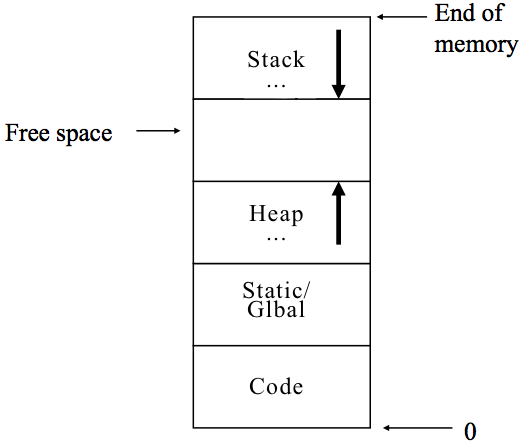
\includegraphics[scale=.6]{mem_management.png}
	\subsection*{Memory areas}
	\begin{itemize}
	\item code: program instructions
	\item global/static: global/static variables
	\item stack: local variables, function arguments, return addresses, temporary storage
	\item heap: dynamically allocated memory
	\end{itemize}
	\subsection*{Stack}
	\begin{itemize}
	\item all variables local to a function and function args stored on the stack
	\item to call func:
		\begin{enumerate}
		\item push args to stack
		\item push return address to stack
		\item jump to function code
		\end{enumerate}
	\item inside function:
		\begin{enumerate}
		\item increment the stack pointer to allow space for the local variables
		\item execute the code
		\item pop local variables and arguments off the stack 
		\item push the return result onto the stack
		\item jump to return address
		\end{enumerate}
	\end{itemize}
	\subsection*{Heap}
	\begin{itemize}
	\item accessed under direct control
	\item request allocation, if there is sufficient contiguous memory available, a pointer is returned to the address of the stage of that memory block
	\end{itemize}
	\subsection*{Memory allocation functions}
	\begin{itemize}
	\item returns a pointer to void 
	\item pointer must be cast to a specific type
	\end{itemize}
	\subsection*{\texttt{malloc}}
	\begin{itemize}
	\item \verb|void *malloc(size_t size)|
	\item requests number of bytes of memory
	\end{itemize}
	\subsection*{\texttt{calloc}}
	\begin{itemize}
	\item \verb|void *calloc(size_t num, size_t size)|
	\item requests number of blocks of memory, and the size of each block
	\item allocated memory is cleared i.e. set to '0'
	\end{itemize}
	\subsection*{\texttt{realloc}}
	\begin{itemize}
	\item \verb|void *realloc(void *ptr, size_t size)|
	\item takes previously allocated memory, and attempts to resize it
	\item contents are preserved
	\item may require new block of memory (for contiguous-ness) $\therefore$ new void pointer is returned
	\end{itemize}
	\subsection*{\texttt{free}}
	\begin{itemize}
	\item \verb|void free(void *ptr)|
	\item deallocates memory previously allocated 
	\item \verb|valgrind|: check for leaks
	\end{itemize}
	\subsection*{to make program happy}
	\begin{itemize}
	\item check memory allocation for success (NULL pointer is returned if unsuccessful)
	\item don't free memory that has already been freed or was never allocated
	\end{itemize}
\end{multicols}

\setcounter{section}{4} % first section is now 2
\hrule
\section{Preprocessor}
\hrule 

\begin{multicols}{2}
	\begin{itemize}
	\item \verb|#include "decs.h"| > copying declarations into every file
	\item useful for externs, tyedefs, struct definitions
	\end{itemize}
	\subsection*{Defined symbols}
	\begin{itemize}
	\item replace identifier with string, everywhere it appears in the program
	\item can be any string of characters, $\therefore$ should bracket arithmetic expressions
	\end{itemize}
	\subsection*{Macros}
	\begin{itemize}
	\item \verb|define min(a,b) ((a) < (b) ? (a) : (b))|
	\end{itemize}
	\subsection*{Conditional inclusion}
	\begin{itemize}
	\item \verb|#ifdef|, \verb|#ifndef|, \verb|#undef|
	\item \verb|#if|, \verb|#elif|, \verb|#else|, \verb|#end|
	\end{itemize}
	\subsection*{Predefined symbols}
	\begin{itemize}
	\item \verb|__LINE__|: current line number at any point
	\item \verb|__FILE__|: name of current program file
	\end{itemize}
	\subsection*{Preprocessor ninjaness}
	\begin{itemize}
	\item \verb|gcc -E| runs only preprocessor
	\item exploit \verb|#define| call by name, and \verb|#ifdef| etc. for conditional generation of hacky templates
	\end{itemize}
	
\end{multicols}

%========================================
% Lecture 6
%========================================

\hrule
\section{Unions and Bitfields}
\hrule 

\begin{multicols}{2}
	\subsection*{Unions}
	\begin{itemize}
	\item variables that occupy the same space
	\item \verb|union {| 
		\\ \hspace*{5mm} \verb|struct {| \\ \hspace*{10mm} \verb|/* struct guts */| \\ \hspace*{5mm} \verb|} type_one;|
		\\ \hspace*{5mm} \verb|struct {| \\ \hspace*{10mm} \verb|/* struct guts */| \\ \hspace*{5mm} \verb|} type_two;|
		\\ \verb|} info;|
	\item access elements: \verb|union_name.part_name|
	\item don't know which variant of the union is being used, $\therefore$ need to use a separate variable to indicate this
	\item \verb|struct catalog x;|
		\\ \verb|switch (x.holding_type) {| 
			\\ \hspace*{5mm} \verb|case book:| \\ \texttt{\hspace*{10mm} <do stuff> \\ \hspace*{10mm} break;}
			\\ \hspace*{5mm} \verb|case film:| \\ \texttt{\hspace*{10mm} <do stuff> \\ \hspace*{10mm} break;}
			\\ \verb|}|
	\end{itemize}
	
% SDNT: bitfields are obvious, can't be bothered writing stuff for it

\end{multicols}

%========================================
% Lecture 7
%========================================

\end{document}